% The relax data model.
%%%%%%%%%%%%%%%%%%%%%%%

\chapter{The relax data model} \label{ch: data model}


% Introduction.
%%%%%%%%%%%%%%%

\section{The concept of the relax data model}

To begin to understand how to use relax, a basic comprehension of the relax data model is needed.
The data model includes the concepts of the relax data store, the data pipes, the molecule, residue and spin data structures and the interatomic data containers.
These concepts are independent of the specific analyses presented in the next chapters and are important for setting up relax.



% The data model.
%%%%%%%%%%%%%%%%%

\section{The data model}


% The relax data store.
%~~~~~~~~~~~~~~~~~~~~~~

\subsection{The relax data store}

All permanent data handled by relax is kept in a structure known as the relax data store.
This structure is initialised when relax is launched.
The data store is primarily organised into a series of objects known as data pipes, and all usage of relax revolves around the flow of information in these data pipes.


% Data pipes.
\subsubsection{Data pipes}

\begin{figure*}[h]
  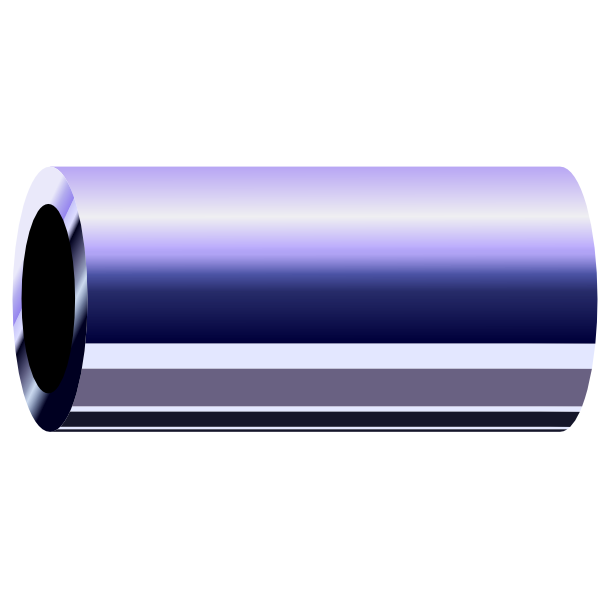
\includegraphics[width=3cm, bb=0 0 1701 1701]{graphics/misc/pipe_600x600}
\end{figure*}

The first thing one must do when relax is launched is to create a data pipe.
When using the GUI, a base data pipe will be created when opening one of the automatic analyses via the analysis selection window (see figure~\ref{fig: screenshot: analysis wizard} on page~\pageref{fig: screenshot: analysis wizard}).
This will also create a data pipe bundle for the analysis (\textit{vide infra}).
Alternatively the data pipe editor window can be used to create data pipes (see figure~\ref{fig: screenshot: pipe editor} on page~\pageref{fig: screenshot: pipe editor}).
For the prompt/scripting modes, or the \guimenuitemthree{User functions}{pipe}{create} menu entry, a data pipe can be initialised by specifying the unique name of the data pipe and the data pipe type:

\begin{lstlisting}
pipe.create(pipe_name='NOE 1200 MHz', pipe_type='noe')
\end{lstlisting}

A number of relax operations will also create data pipes by merging a group of pipes or branching pre-existing pipes.
See section~\ref{sect: the data pipe} on page~\pageref{sect: the data pipe} for additional details.

All data not associated with spin systems will be stored in the base data pipe.
This includes information such as global optimisation statistics, diffusion tensors, alignment tensors, 3D structural data, the molecule, residue and spin container data structure and the interatomic data containers.
One data pipe from the set will be defined as being the current data pipe, and all operations in relax will effect data from this pipe.
The \uf{pipe\ufsep{}switch} user function in all UI modes can be used to change which pipe is the current data pipe.
In the GUI, switching between analysis tabs will automatically switch the current data pipe to match the analysis being displayed.


% Data pipe bundles.
\subsubsection{Data pipe bundles} \label{sect: data pipe bundles}

\begin{figure*}[h]
  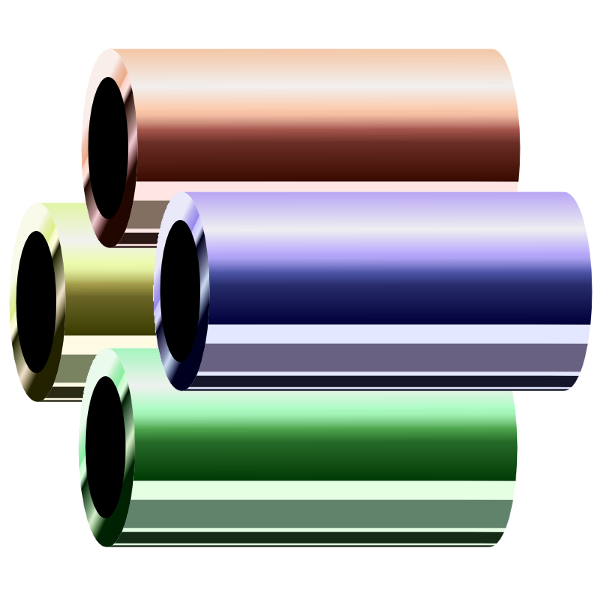
\includegraphics[width=3cm, bb=0 0 1701 1701]{graphics/misc/pipe_bundle_600x600}
\end{figure*}

Related data pipes can be grouped into a `bundle'.
For example if the data pipes ``sphere'', ``oblate spheroid'', ``prolate spheroid'', and ``ellipsoid'' preexist, these can be grouped into a bundle called ``diffusion tensors'' with the following series of user function calls:

\begin{lstlisting}
pipe.bundle(bundle='diffusion tensors', pipe='sphere')
pipe.bundle(bundle='diffusion tensors', pipe='oblate spheroid')
pipe.bundle(bundle='diffusion tensors', pipe='prolate spheroid')
pipe.bundle(bundle='diffusion tensors', pipe='ellipsoid')
\end{lstlisting}

The data pipe editor window of the GUI can also be used to bundle pipes together (see figure~\ref{fig: screenshot: pipe editor} on page~\pageref{fig: screenshot: pipe editor}).



% Molecule, residue, and spin containers.
%~~~~~~~~~~~~~~~~~~~~~~~~~~~~~~~~~~~~~~~~

\subsection{Molecule, residue, and spin containers}

Within a data pipe is the molecule, residue, and spin container data structure.
Data which is specific to a given nucleus is stored in a special spin container structure.
This includes relaxation data, model-free parameters, reduced spectral density mapping values, spin specific optimisation parameters, chemical shift tensor information, pseudo-contact shift values, etc.
The spin containers can be created from 3D structural data or a sequence file, as described in the next two sections, or manually built.



% Molecule containers.
\subsubsection{Molecule containers}

\begin{figure*}[h]
  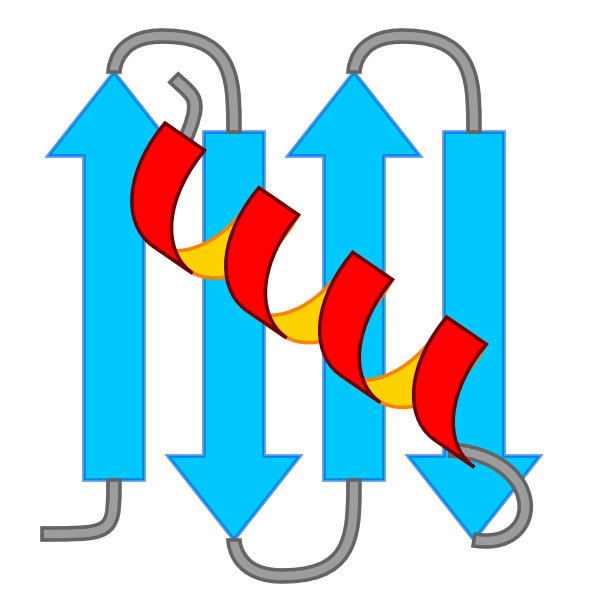
\includegraphics[width=3cm, bb=0 0 1701 1701]{graphics/misc/molecule_600x600}
\end{figure*}

The spin containers are part of a nested set of containers, and are graphically depicted in the spin viewer window of the GUI in figure~\ref{fig: screenshot: spin viewer} on page~\pageref{fig: screenshot: spin viewer}.
As can be seen from the figure, the top level holds a single molecular container.
Multiple molecular containers can be present if the study is of a molecular complex.
Using the GUI menus or the prompt/scripting mode, molecule containers can be manually created with the user function:

\begin{lstlisting}
molecule.create(mol_name='glycerol', mol_type='organic molecule')
\end{lstlisting}

In the spin viewer window of the GUI, right clicking on the \gui{Spin system information} element will pop up a menu with an entry for adding molecule containers.
Right clicking on molecule containers will show a pop up menu with an entry for permanently deleting the container.



% Residue containers.
\subsubsection{Residue containers}

\begin{figure*}[h]
  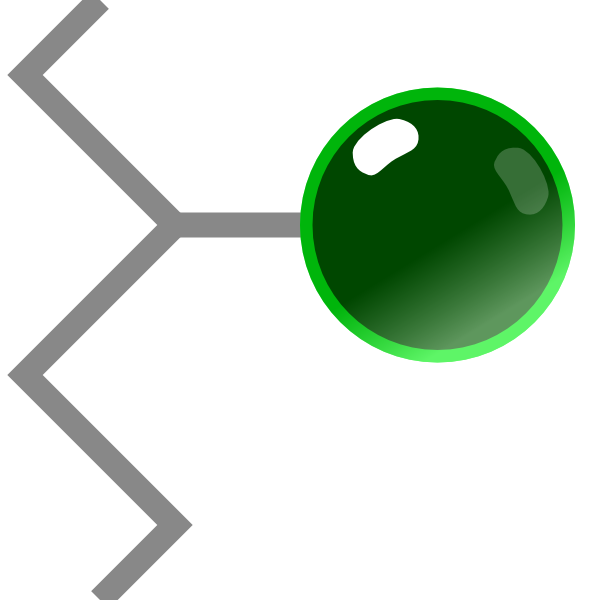
\includegraphics[width=3cm, bb=0 0 1701 1701]{graphics/misc/residue_600x600}
\end{figure*}

Nested within the molecule containers are residue containers.
These are graphically depicted in the spin viewer window (see figure~\ref{fig: screenshot: spin viewer} on page~\pageref{fig: screenshot: spin viewer}).
Each molecule container can possess multiple residues.
These require either a unique residue number or unique residue name.
For organic molecules where the residue concept is meaningless, all spin containers can be held within a single unnamed and unnumbered residue container.
Using the GUI menus or the prompt/scripting mode, residue containers can be manually created with the user function:

\begin{lstlisting}
residue.create(res_num='-5', res_name='ASP')
\end{lstlisting}

Alternatively residues can be added in the spin viewer window from the pop up menu when right clicking on molecule containers, and can be deleted via the pop up menu when right clicking on the residue to delete.



% Spin containers.
\newpage
\subsubsection{Spin containers}

\begin{figure*}[h]
  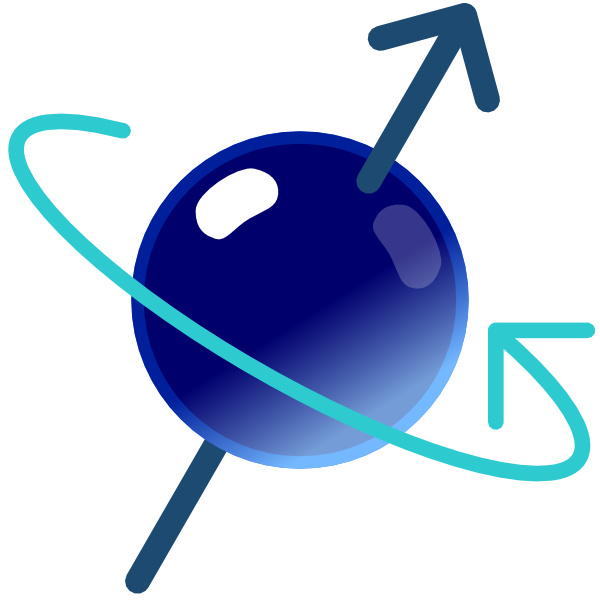
\includegraphics[width=3cm, bb=0 0 1701 1701]{graphics/misc/spin_600x600}
\end{figure*}

Spin containers are nested within a residue container (again graphically depicted in the spin viewer window in figure~\ref{fig: screenshot: spin viewer} on page~\pageref{fig: screenshot: spin viewer}).
Multiple spin containers can exist per residue.
This allows, for example, a single model-free analysis simultaneously on the backbone nitrogen spins, side-chain tryptophan indole nitrogen spins and alpha carbon spins.
Or, for example, studying the pseudocontact shifts for all nitrogen, carbon and proton spins in the molecule simultaneously.

Spin containers can be manually added via the \uf{spin\ufsep{}create} user function in the GUI or prompt/scripting mode:

\begin{lstlisting}
spin.create(spin_num='200', spin_name='NE1')
\end{lstlisting}

The spin viewer window can also be used by right clicking on residue containers.



% Spin ID strings.
\subsubsection{Spin ID strings} \label{sect: spin ID}

Spins are often identified in relax using their ID strings.
The spin ID strings follow the basic construct found in a number of other NMR software such as MOLMOL.
The identification string is composed of three components:
\begin{itemize}
  \item The molecule ID token beginning with the \promptstring{\#} character,
  \item The residue ID token beginning with the \promptstring{:} character,
  \item The atom or spin system ID token beginning with the \promptstring{@} character.
\end{itemize}

Each token can be composed of multiple elements -- one per spin -- separated by the \promptstring{,} character and each individual element can either be a number (which must be an integer, in string format), a name, or a range of numbers separated by the \promptstring{-} character.
Negative numbers are supported.
The full ID string specification is \promptstring{\#<mol\_name> :<res\_id>[, <res\_id>[, <res\_id>, ...]] @<atom\_id>[, <atom\_id>[, <atom\_id>, ...]]}, where the token elements are \promptstring{<mol\_name>}, the name of the molecule, \promptstring{<res\_id>}, the residue identifier which can be a number, name, or range of numbers, \promptstring{<atom\_id>}, the atom or spin system identifier which can be a number, name, or range of numbers.

If one of the tokens is left out then all elements will be assumed to match.
For example if the string does not contain the \promptstring{\#} character then all molecules will match the string.
If only the molecule ID component is specified, then all spins of the molecule will match.

Regular expression can, in some instances, be used to select spins.
For example the string \promptstring{@H*} will select the protons `H', `H2' and `H98'.



% Interatomic data containers.
%%%%%%%%%%%%%%%%%%%%%%%%%%%%%%

\section{Interatomic data containers} \label{sect: interatomic container}

\begin{figure*}[h]
  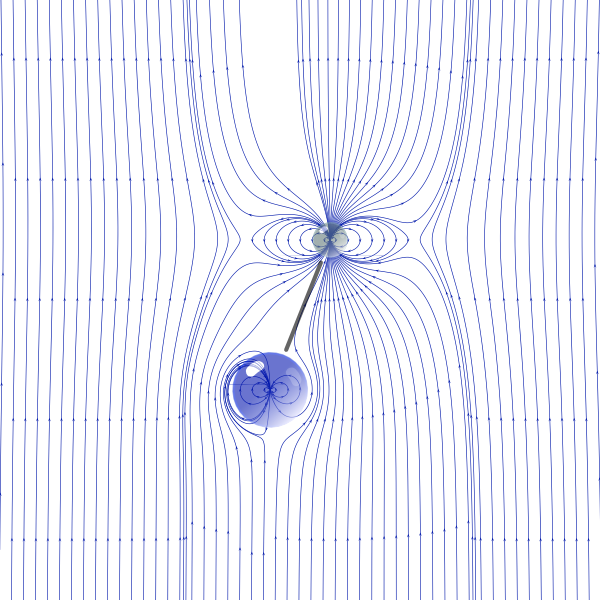
\includegraphics[width=3cm, bb=0 0 1701 1701]{graphics/wizards/dipole_pair/NH_dipole_pair_600x600}
\end{figure*}

Separate from the spin containers, yet strongly linked to them, are the interatomic data containers.
These containers are grouped together within the same data pipe as the spins they point to.
These define interactions between two spins located anywhere within the molecule, residue and spin nested data structure.
These are automatically created when reading in data defined between two spins such as RDCs and NOE distance constraints.
They can also be created using the \uf{interatom\ufsep{}define} user function:

\begin{lstlisting}
interatom.define(spin_id1=':2@N', spin_id2=':2@H')
\end{lstlisting}

As the interatomic data container concept is relatively new, how they are created and handled is likely to evolve and change in the future.



% Setup in the prompt/script UI.
%%%%%%%%%%%%%%%%%%%%%%%%%%%%%%%%

\section{Setup in the prompt/script UI}

Below are three different examples showing how to set up the relax data model for any analysis type requiring spin specific data.


% Spins from structural data.
%~~~~~~~~~~~~~~~~~~~~~~~~~~~~

\subsection{Script mode -- spins from structural data} \label{sect: script - structural data}

\begin{figure*}[h]
  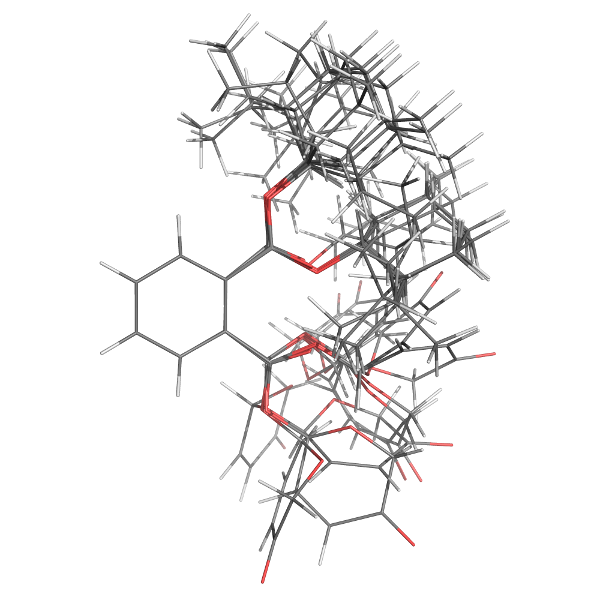
\includegraphics[width=3cm, bb=0 0 1701 1701]{graphics/misc/n_state_model/phthalic_acid_ens_600x600}
\end{figure*}

3D structural data is stored at the level of the current data pipe.
This data is completely separate from the molecule, residue and spin data structure.
However the structural data can be used to generate the spin containers.
For example for the nitrogen relaxation in a model-free analysis where both the nitrogen and proton are needed to define the magnetic dipole-dipole relaxation:

\begin{lstlisting}
# Create a data pipe.
pipe.create(pipe_name='ellipsoid', pipe_type='mf')

# Load the PDB file.
structure.read_pdb('1f3y.pdb')

# Set up the 15N and 1H backbone spins.
structure.load_spins('@N', ave_pos=True)
structure.load_spins('@H', ave_pos=True)

# Set up the 15N and 1H for the tryptophan indole ring.
structure.load_spins('@NE1', ave_pos=True)
structure.load_spins('@HE1', ave_pos=True)

# Define the spin isotopes.
spin.isotope('15N', spin_id='@N*')
spin.isotope('1H', spin_id='@H*')
\end{lstlisting}

The \uf{structure\ufsep{}read\ufus{}pdb} user function will load the structural data into the current data pipe, and the \uf{structure\ufsep{}load\ufus{}spins} user function will create the molecule, residue, and spin containers as needed.
This will also load atomic position information into the matching spin containers.
The \uf{spin\ufsep{}isotope} user function is required to define the magnetic dipole-dipole interaction and is information not present in the PDB file.

Note that if structural data from the PDB is used to generate the spin containers, then all subsequent data loaded into relax must follow the exact naming convention from the PDB file.
Automatic residue name matching (i.e.\ `GLY' = `Gly' = `gly' = `G') is currently not supported.



% Spins from a sequence file.
%~~~~~~~~~~~~~~~~~~~~~~~~~~~~

\subsection{Script mode -- spins from a sequence file} \label{sect: script - sequence file}

\begin{figure*}[h]
  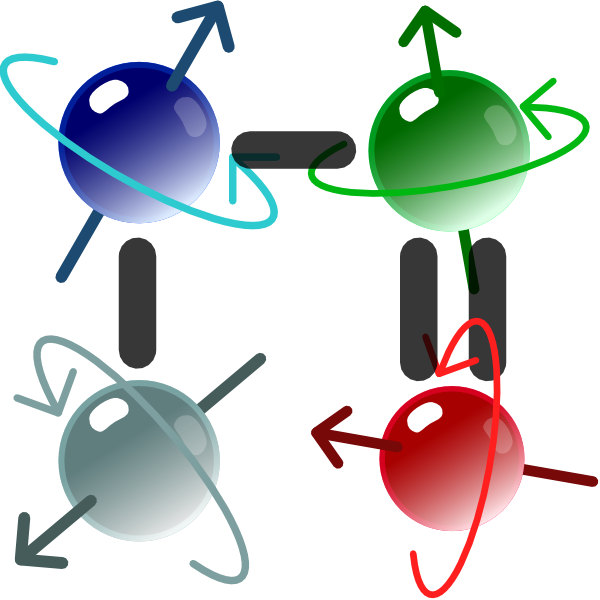
\includegraphics[width=3cm, bb=0 0 1701 1701]{graphics/misc/sequence_600x600}
\end{figure*}

Alternatively to setting up the molecule, residue, and spin containers via 3D structural data, a plain text columnar formatted file can be used.
This is useful for when no 3D structure exists for the molecule.
It also has the advantage that the residue and atom names need not conform to the PDB standard.
An example for reading sequence data is:

\begin{lstlisting}
# Create a data pipe.
pipe.create(pipe_name='R1 1200', pipe_type='relax_fit')

# Set up the 15N spins.
sequence.read(file='noe.500.out', mol_name_col=1, res_num_col=2, res_name_col=3, spin_num_col=4, spin_name_col=5)
spin.element(element='N', spin_id='@N*')
spin.isotope('15N', spin_id='@N')
\end{lstlisting}

Here the molecule, residue, and spin information is extracted from the \promptstring{noe.500.out} file which could look like:

{\scriptsize \begin{verbatim}
# mol_name          res_num  res_name  spin_num  spin_name  value             error               
Ap4Aase_new_3_mol1  1        GLY       1         N          None              None                
Ap4Aase_new_3_mol1  2        PRO       11        N          None              None                
Ap4Aase_new_3_mol1  3        LEU       28        N          None              None                
Ap4Aase_new_3_mol1  4        GLY       51        N          0.03892194698453  0.01903177024613    
Ap4Aase_new_3_mol1  5        SER       59        N          0.31240422567912  0.01859693729836    
Ap4Aase_new_3_mol1  6        MET       71        N          0.42850831873249  0.0252585632304     
Ap4Aase_new_3_mol1  7        ASP       91        N          0.53054928103134  0.02799062314416    
Ap4Aase_new_3_mol1  8        SER       104       N          0.56528429775819  0.02170612146773    
Ap4Aase_new_3_mol1  9        PRO       116       N          None              None                
Ap4Aase_new_3_mol1  40       TRP       685       N          0.65394813490548  0.03830061886537    
Ap4Aase_new_3_mol1  40       TRP       698       NE1        0.67073879732046  0.01426066343831    
\end{verbatim}} \label{verb: noe.500.out}

The file can contain columns for the molecule name, the residue name and number, and the spin name and number in any order though not all are needed.
For example for a single protein system, the molecule name, residue name and spin number are nonessential.
Or for an organic molecule, the molecule name, residue name and number and spin number could be nonessential.
The subsequent user functions in the above example are used to set up the spin containers appropriately for a model-free analysis.
These are not required in the automatic analysis of GUI as these user functions will be presented to you when adding relaxation data, or when clicking on the heteronucleus and proton buttons (\guibutton{X isotope} and \guibutton{H isotope}).

In the GUI, the creation of molecule, residue, and spin containers from a sequence file is also available via the \gui{Load spins} wizard within the spin viewer window (\textit{vide supra}).


% Manual construction.
%~~~~~~~~~~~~~~~~~~~~~

\subsection{Script mode -- manual construction} \label{sect: script - manual construction}

For the masochists out there, the full molecule, residue and spin data structure can be manually constructed.
For example:

\begin{lstlisting}
# Manually create the molecule, residue, and spin containers.
molecule.create(mol_name='Ap4Aase', mol_type='protein')
residue.create(res_num=1,  res_name='GLY')
residue.create(res_num=3,  res_name='LEU')
residue.create(res_num=96, res_name='TRP')
spin.create(res_num=1,  spin_name='N')
spin.create(res_num=3,  spin_name='N')
spin.create(res_num=96, spin_name='N')
spin.create(res_num=96, spin_name='NE1')
\end{lstlisting}

These user functions can be repeated until the full sequence has been constructed.



% Setup in the GUI.
%%%%%%%%%%%%%%%%%%%

\section{Setup in the GUI}


% The data pipe.
%~~~~~~~~~~~~~~~

\subsection{GUI mode -- setting up the data pipe} \label{sect: GUI - data pipe}

In the GUI, the most common way to create the data pipe is to initialise one of the auto-analyses via the analysis selection wizard (see Figure~\ref{fig: screenshot: analysis wizard} on page~\pageref{fig: screenshot: analysis wizard}).
The initialisation will create the appropriate starting data pipe.
Alternatively the data pipe editor can be used (see Figure~\ref{fig: screenshot: pipe editor} on page~\pageref{fig: screenshot: pipe editor}).
Or the \guimenuitemthree{User functions}{pipe}{create} menu item can be selected for graphical access to the \uf{pipe\ufsep{}create} user function.



% Spins from structural data.
%~~~~~~~~~~~~~~~~~~~~~~~~~~~~

\subsection{GUI mode -- spins from structural data} \label{sect: GUI - structural data}

For this section, the example of protein $^{15}$N relaxation data will be used to illustrate how to set up the data structures.
To manipulate the molecule, residue and spin data structures in the GUI, the most convenient option is to use the spin viewer window (see Figure~\ref{fig: screenshot: spin viewer} on page~\pageref{fig: screenshot: spin viewer}).
This window can be opened in four ways:
\begin{itemize}
  \item The \guimenuitemtwo{View}{Spin viewer} menu item,
  \item The \shortcutkey{Ctrl+T} key combination,
  \item The spin viewer icon in the toolbar (represented by the blue spin icon),
  \item The \guibutton{Spin editor} button part of the \gui{Spin systems} GUI element in the specific analysis tabs.
\end{itemize}

You will then see:

\begin{minipage}[h]{\linewidth}
  \centerline{
    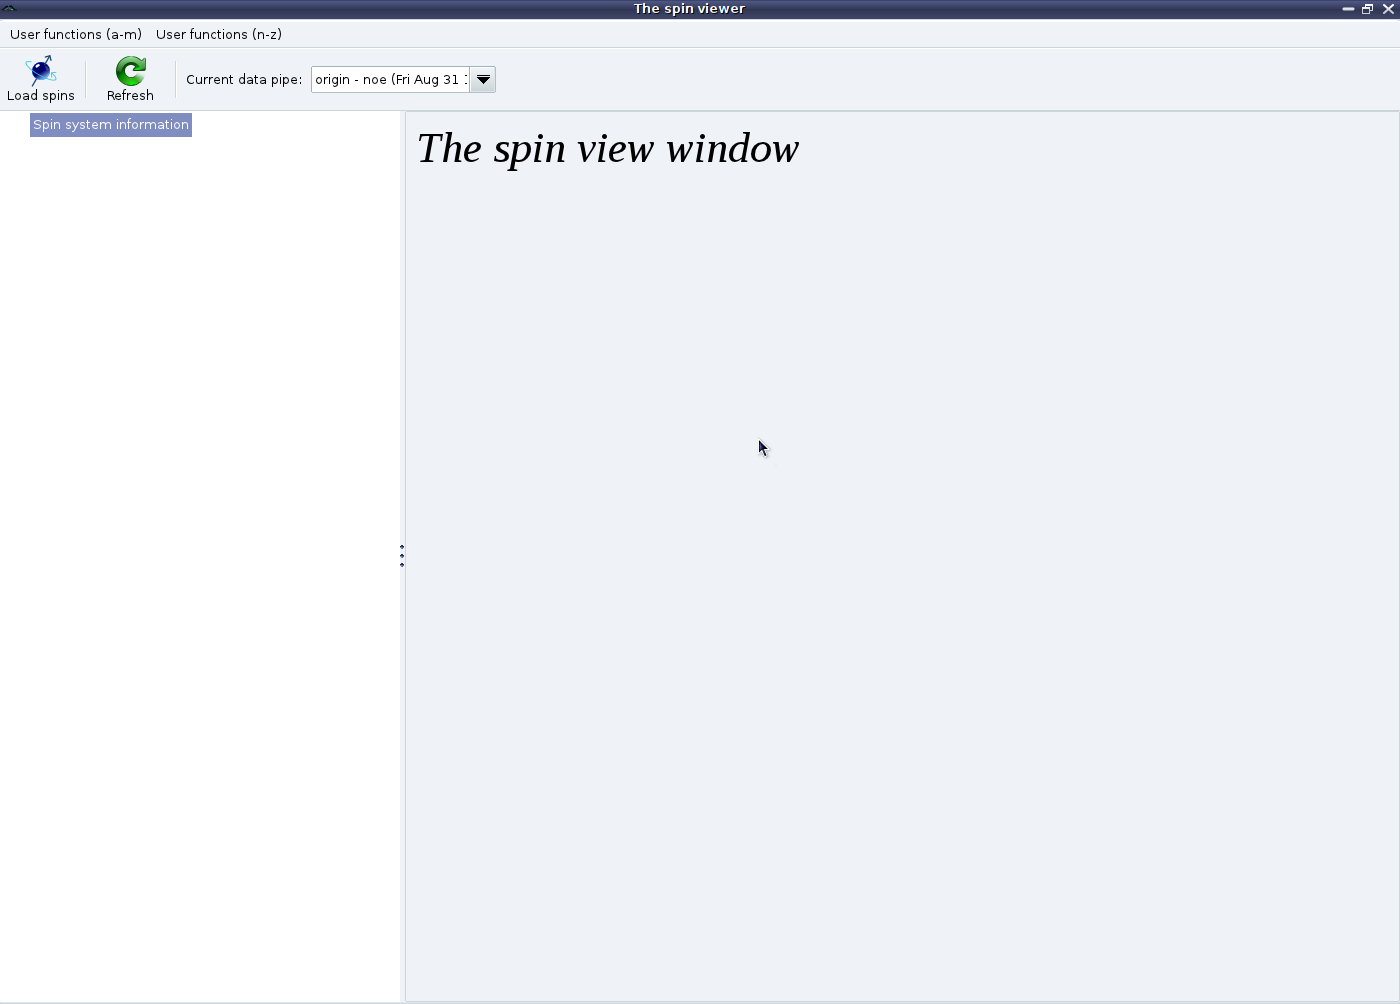
\includegraphics[
      width=0.8\textwidth,
      bb=14 14 1415 1019
    ]
    {graphics/screenshots/spin_viewer/blank}
  }
  \label{figure: spin viewer blank}
\end{minipage}

At this point, click on the \guibutton{Load spins} button (or the \guimenuitemone{Load spins} menu entry from the right click pop up menu) to launch the spin loading wizard.
A number of options will be presented to you: 

\begin{minipage}[h]{\linewidth}
  \centerline{
    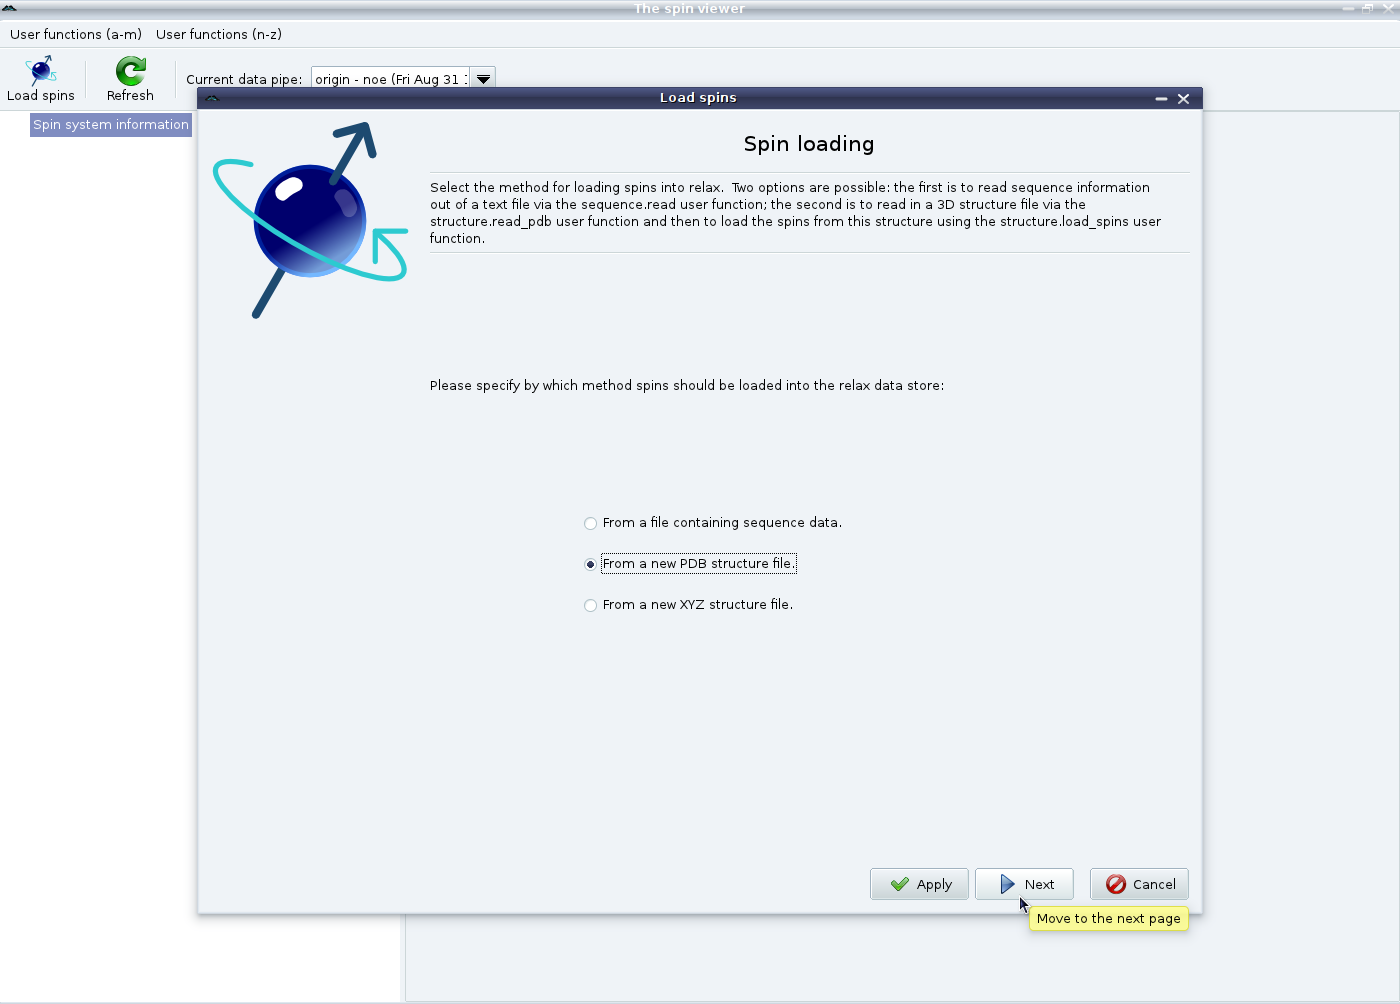
\includegraphics[
      width=0.8\textwidth,
      bb=14 14 1415 1019
    ]
    {graphics/screenshots/spin_viewer/wizard_start}
  }
  \label{figure: spin viewer wizard start}
\end{minipage}

Here the spins will be loaded from a PDB file.
If you do not have a 3D structure file, please see the next section.
After selecting \gui{From a new PDB structure file} and clicking on \guibutton{Next}, you will see:

\begin{minipage}[h]{\linewidth}
  \centerline{
    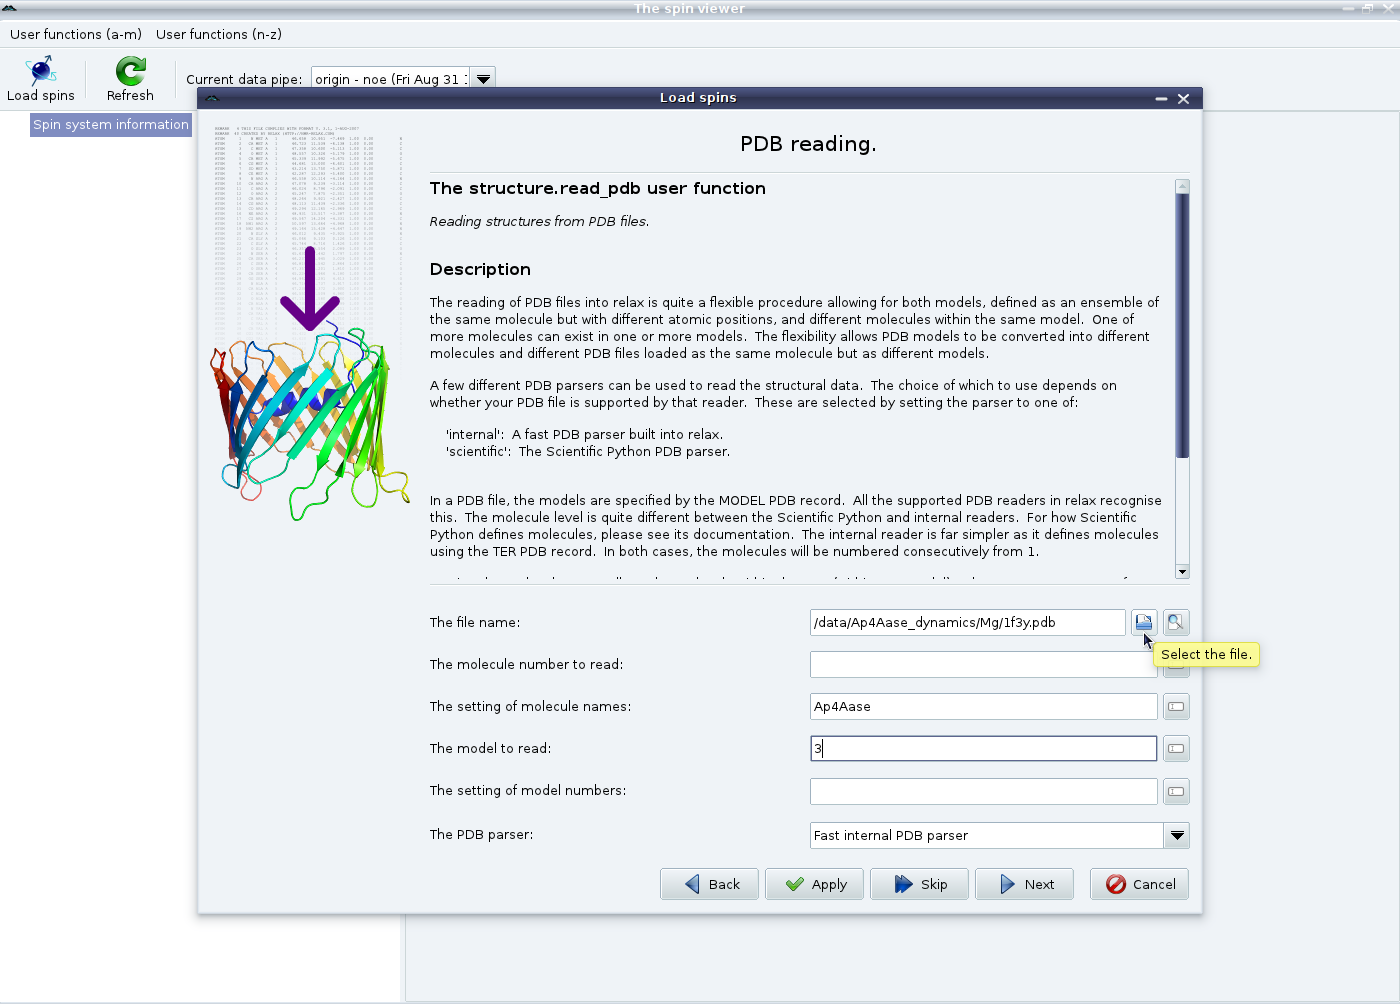
\includegraphics[
      width=0.8\textwidth,
      bb=14 14 1415 1019
    ]
    {graphics/screenshots/spin_viewer/wizard_read_pdb}
  }
\end{minipage}

Now select the PDB file you wish to use.
The other options in this screen allow you to handle NMR models and multiple molecules within a single PDB file.
These options are explained in the window.
Hovering the mouse over the options will give additional hints.
In this example, the \nth{3} model from the 1F3Y PDB file will be read and the single molecule will be named \guistring{Ap4Aase} to override the default naming of \guistring{1f3y\_mol1}.
Now click on \guibutton{Next} to bring up the spin loading page:

\begin{minipage}[h]{\linewidth}
  \centerline{
    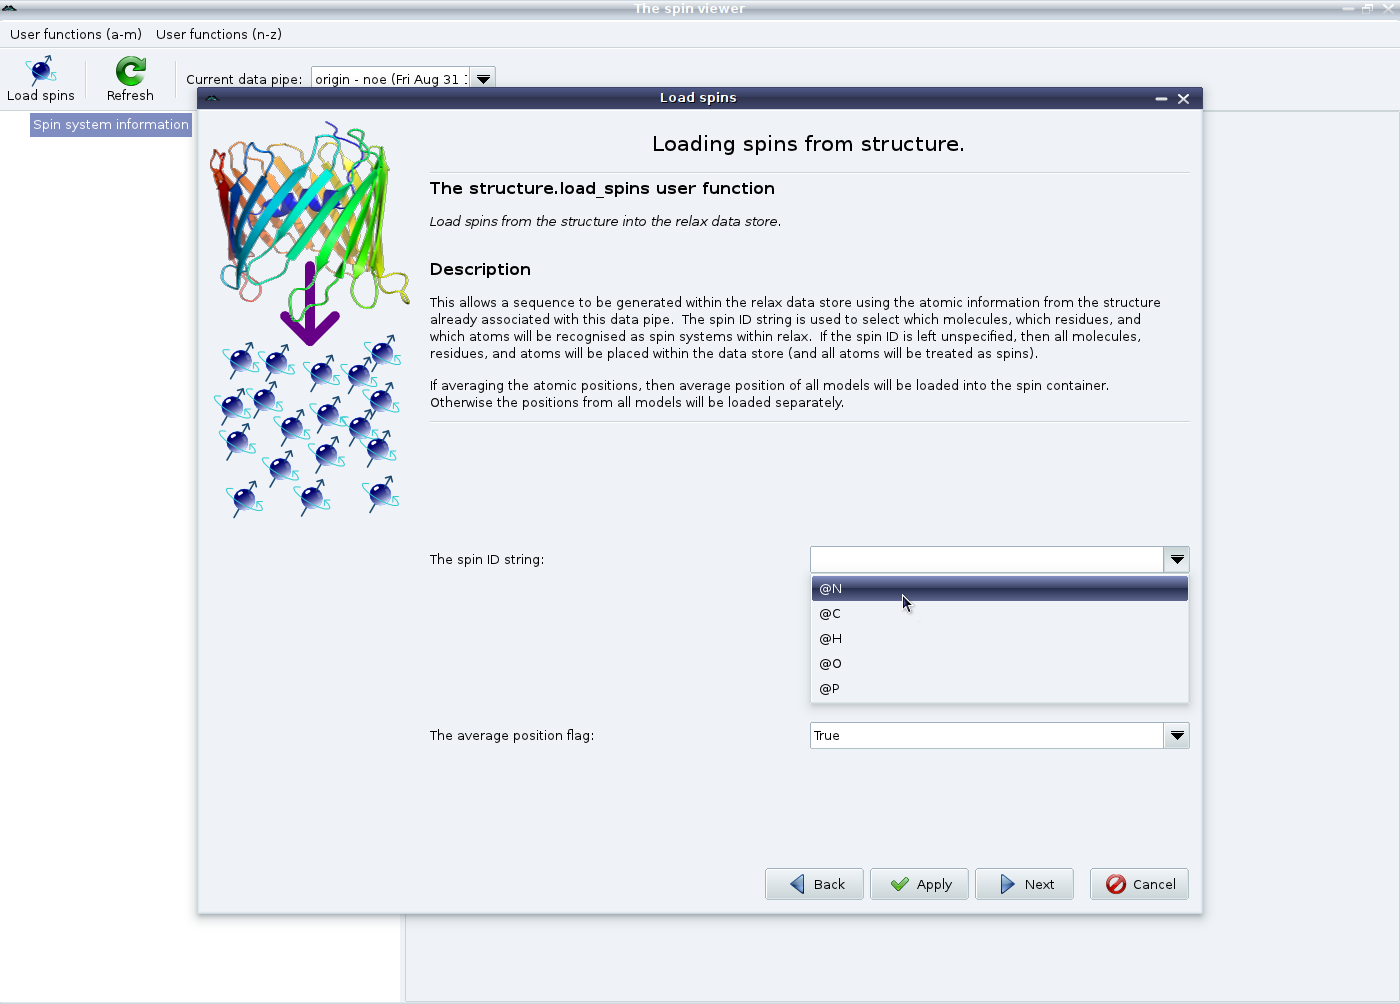
\includegraphics[
      width=0.8\textwidth,
      bb=14 14 1415 1019
    ]
    {graphics/screenshots/spin_viewer/wizard_load_spins_n}
  }
\end{minipage}

This is a bit more complicated.
In this example we are studying the backbone dynamics of $^{15}$N spins of a protein.
Therefore first set the spin ID string to \guistring{@N} (which can be selected from the pull down) and click on \guibutton{Apply} to set up the backbone spins.
Do not click on \guibutton{Next} yet.
If the current study requires the specification of the dipole-dipole interaction (for example if it involves relaxation data -- model-free analyses, consistency testing, reduced spectral density mapping; or the dipolar coupling -- the N-state model or ensemble analyses, the Frame Order theory) you will also need to load the $^1$H spins as well.
Therefore set the spin ID string to \guistring{@H} and click on \guibutton{Apply} again.


\begin{minipage}[h]{\linewidth}
  \centerline{
    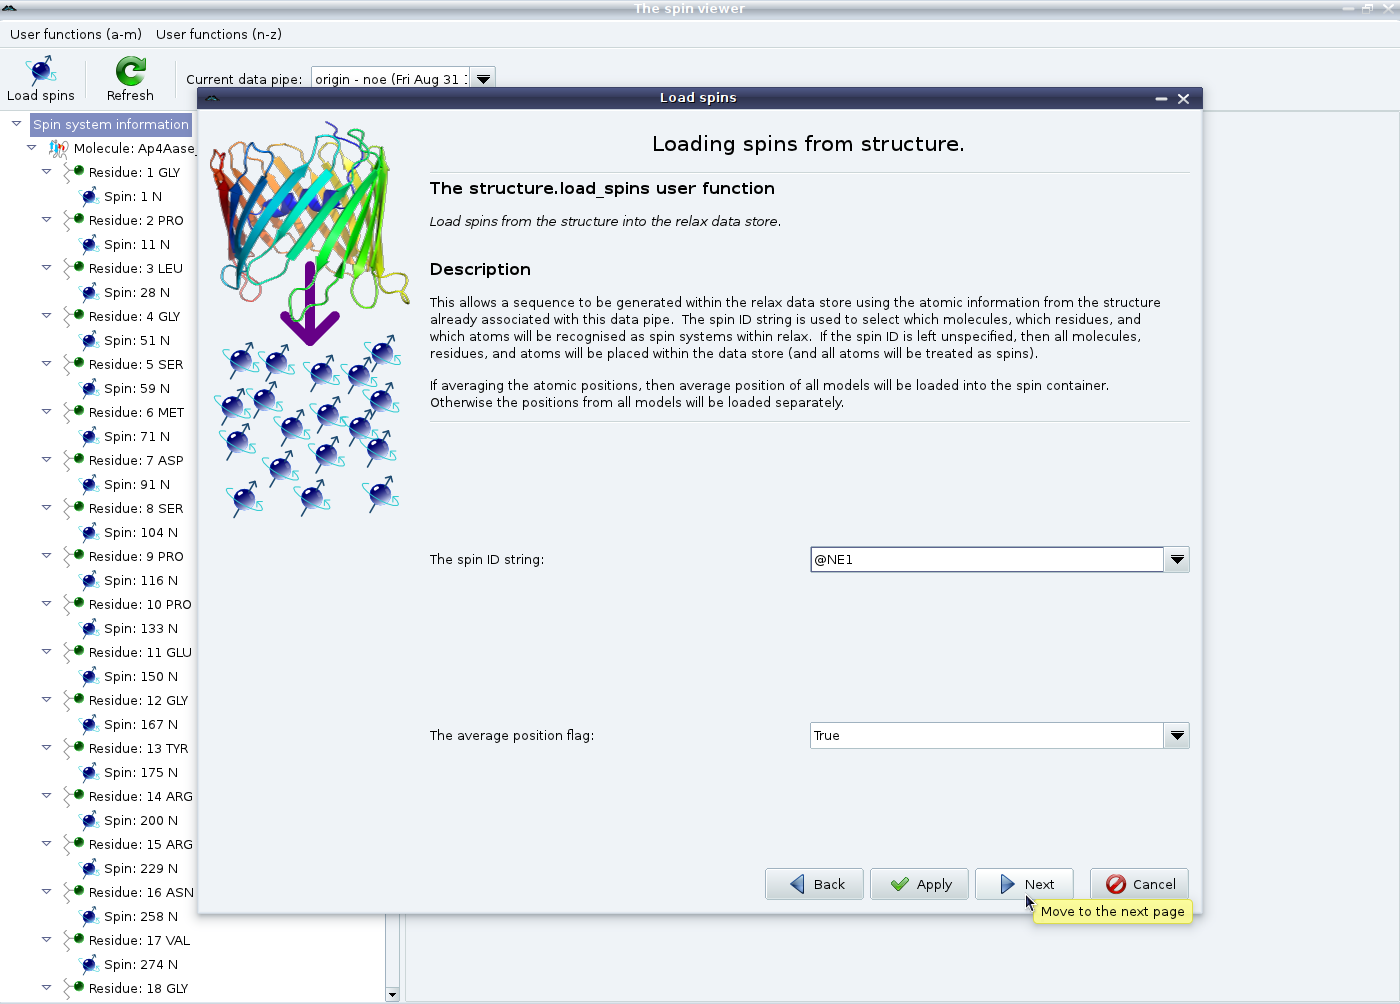
\includegraphics[
      width=0.8\textwidth,
      bb=14 14 1415 1019
    ]
    {graphics/screenshots/spin_viewer/wizard_load_spins_ne1}
  }
\end{minipage}

Now change the spin ID string to \guistring{@NE1} and then click on \guibutton{Next} (or \guibutton{Apply} if the Trp protons \guistring{@HE1} need to be loaded as well).
This will add spin containers for the tryptophan indole $^{15}$N spins.
Finally click on \guibutton{Finish} to exit the wizard:

\begin{minipage}[h]{\linewidth}
  \centerline{
    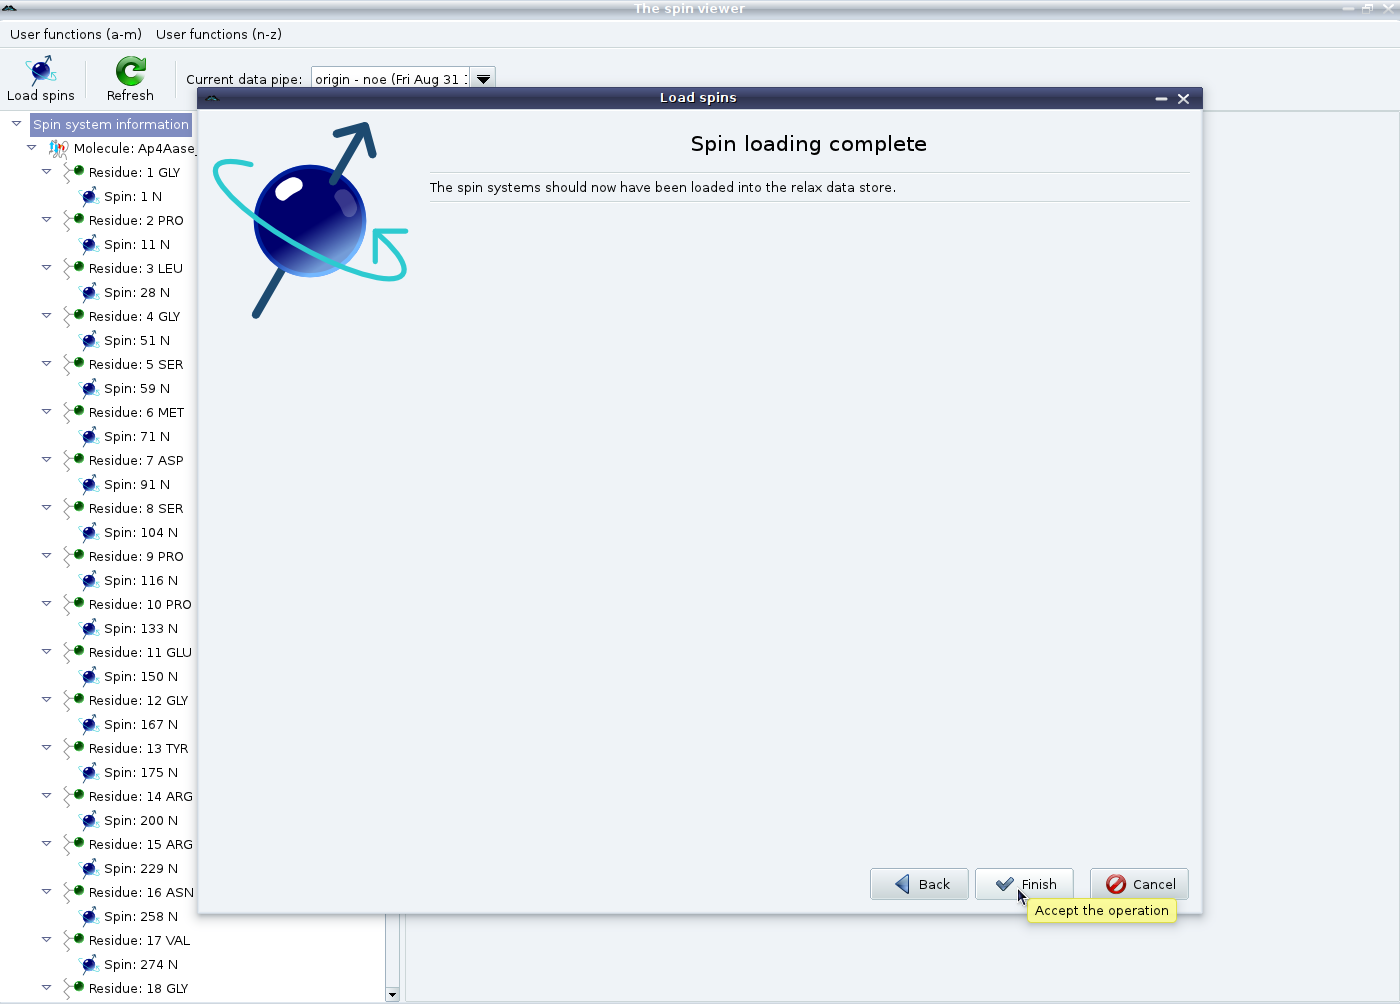
\includegraphics[
      width=0.8\textwidth,
      bb=14 14 1415 1019
    ]
    {graphics/screenshots/spin_viewer/wizard_end}
  }
\label{figure: spin viewer end}
\end{minipage}

You should now see something such as:

\begin{minipage}[h]{\linewidth}
  \centerline{
    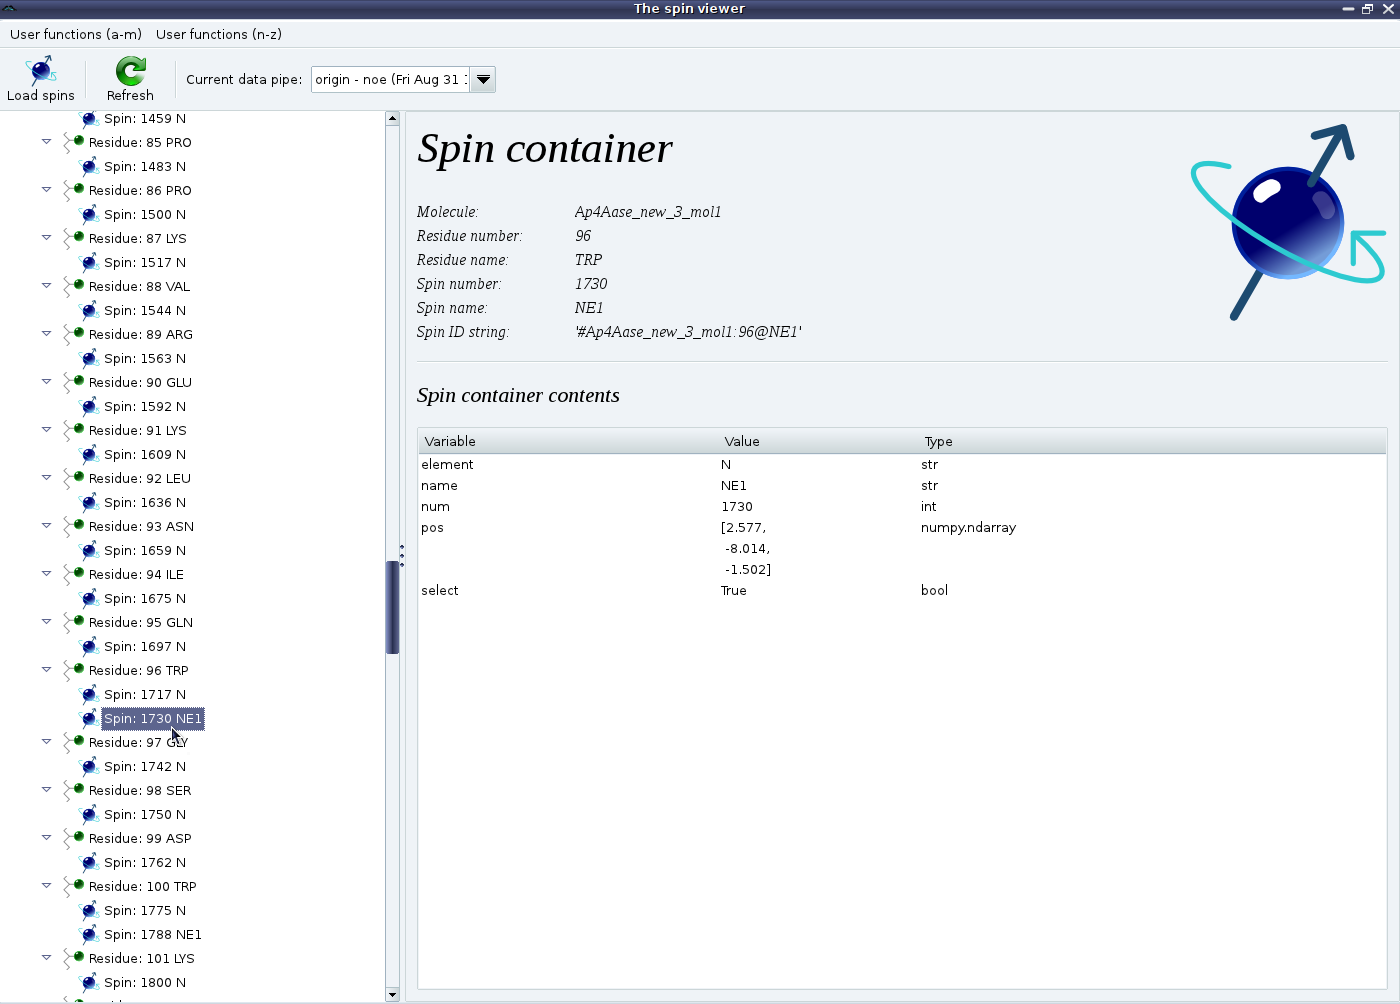
\includegraphics[
      width=0.8\textwidth,
      bb=14 14 1415 1019
    ]
    {graphics/screenshots/spin_viewer/full}
  }
\end{minipage}

If the $^1$H spins have been loaded as well, then you should see exactly twice as many spin containers as shown above.


% Spins from a sequence file.
%~~~~~~~~~~~~~~~~~~~~~~~~~~~~

\subsection{GUI mode -- spins from a sequence file} \label{sect: GUI - sequence file}

Starting from the empty spin viewer window on page~\pageref{figure: spin viewer blank}), click on the \guibutton{Load spins} button.
You will then see the spin loading wizard (see page~\pageref{figure: spin viewer wizard start}).
Select the option for reading data from a sequence file.
You should then see:

\begin{minipage}[h]{\linewidth}
  \centerline{
    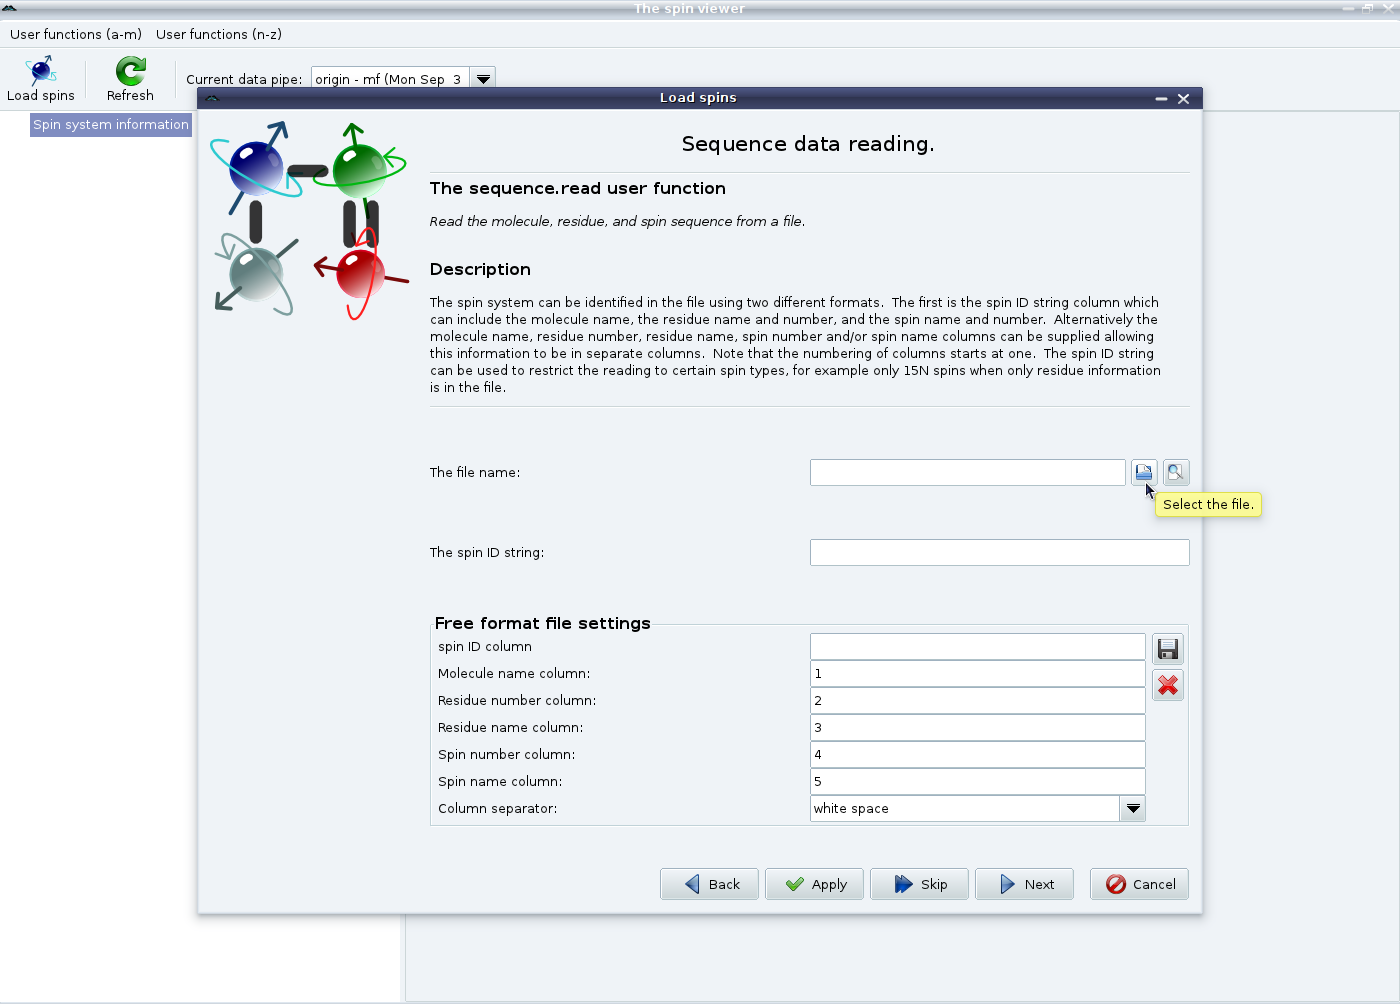
\includegraphics[
      width=0.8\textwidth,
      bb=14 14 1415 1019
    ]
    {graphics/screenshots/spin_viewer/wizard_sequence}
  }
\end{minipage}

Select the file to load and change the \gui{Free format file settings} as needed.
An example of a suitable format is given on page~\pageref{verb: noe.500.out}.
Click on \guibutton{Next} to reach the wizard ending page (see~\pageref{figure: spin viewer end}).
Finally click on \guibutton{Finish} to exit the wizard.


% Manual construction.
%~~~~~~~~~~~~~~~~~~~~~

\subsection{GUI mode -- manual construction} \label{sect: GUI - manual construction}

Just as in the prompt/script UI mode, the molecules, residues and spins can be manually added.
First add a molecule by right clicking on the \gui{Spin system information} element and selecting the relevant entry in the popup menu.
Then right click on the newly created molecule container to add residues, and right click on residue containers to add spins.


% Deselect spins.
%~~~~~~~~~~~~~~~~

\subsection{GUI mode -- deselect spins} \label{sect: GUI - deselect spins}

To deselect spins (for example if they are unresolved, overlapping peaks), click on the \guimenuitemthree{User functions}{deselect}{read} menu item from the main relax window or the spin viewer window:

\begin{minipage}[h]{\linewidth}
  \centerline{
    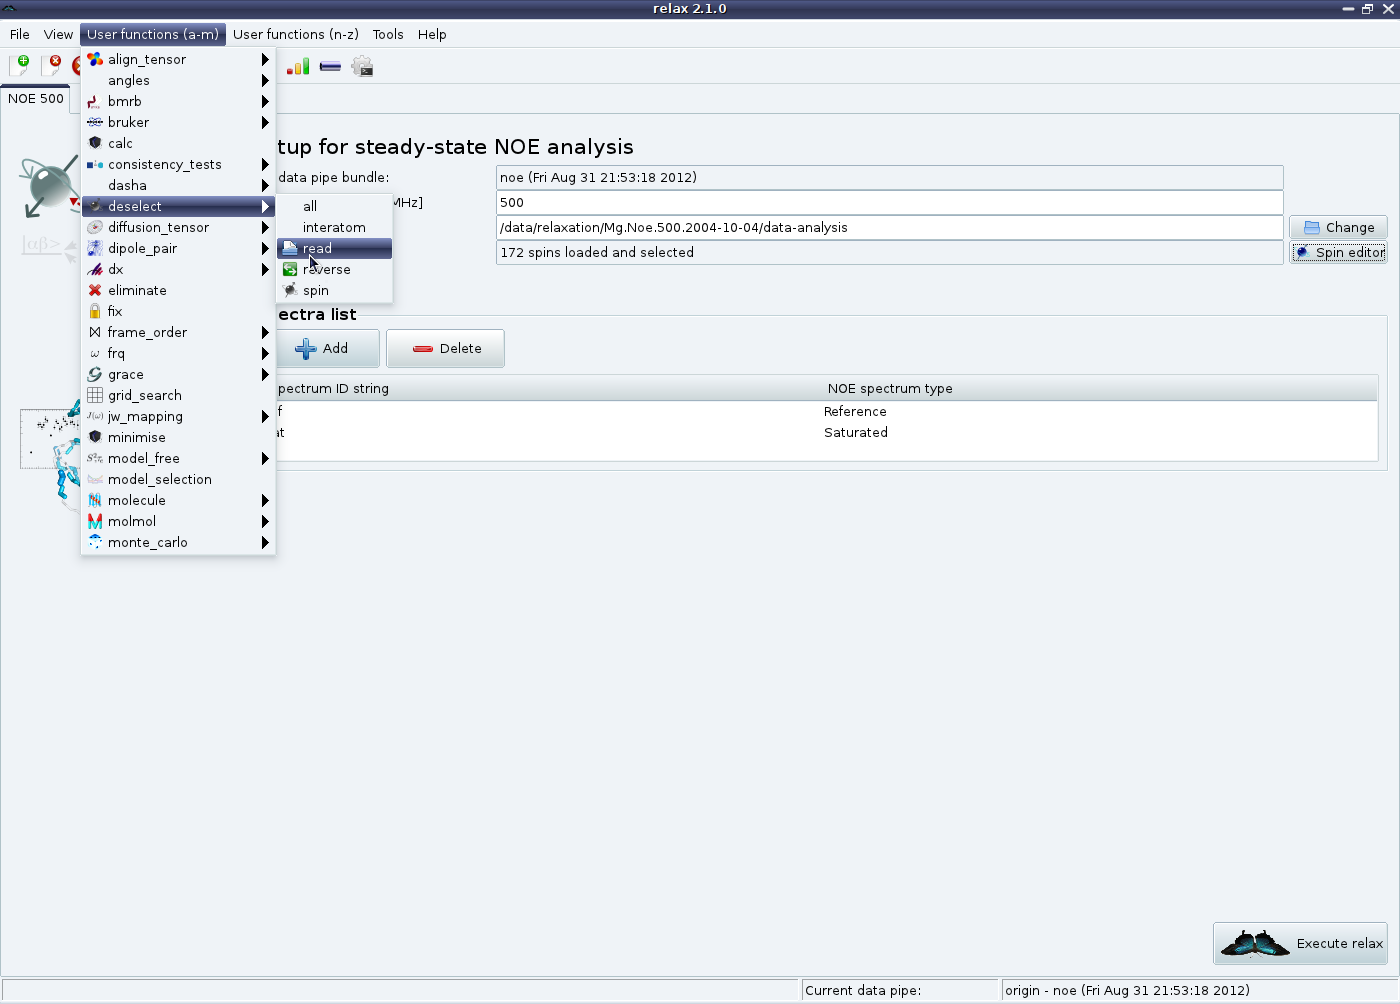
\includegraphics[
      width=0.8\textwidth,
      bb=14 14 1415 1019
    ]
    {graphics/screenshots/noe_analysis/analysis_tab3}
  }
\end{minipage}

Select the file listing the unresolved spins and change the column numbers in the \gui{Free format file settings} GUI element as needed: 

\begin{minipage}[h]{\linewidth}
  \centerline{
    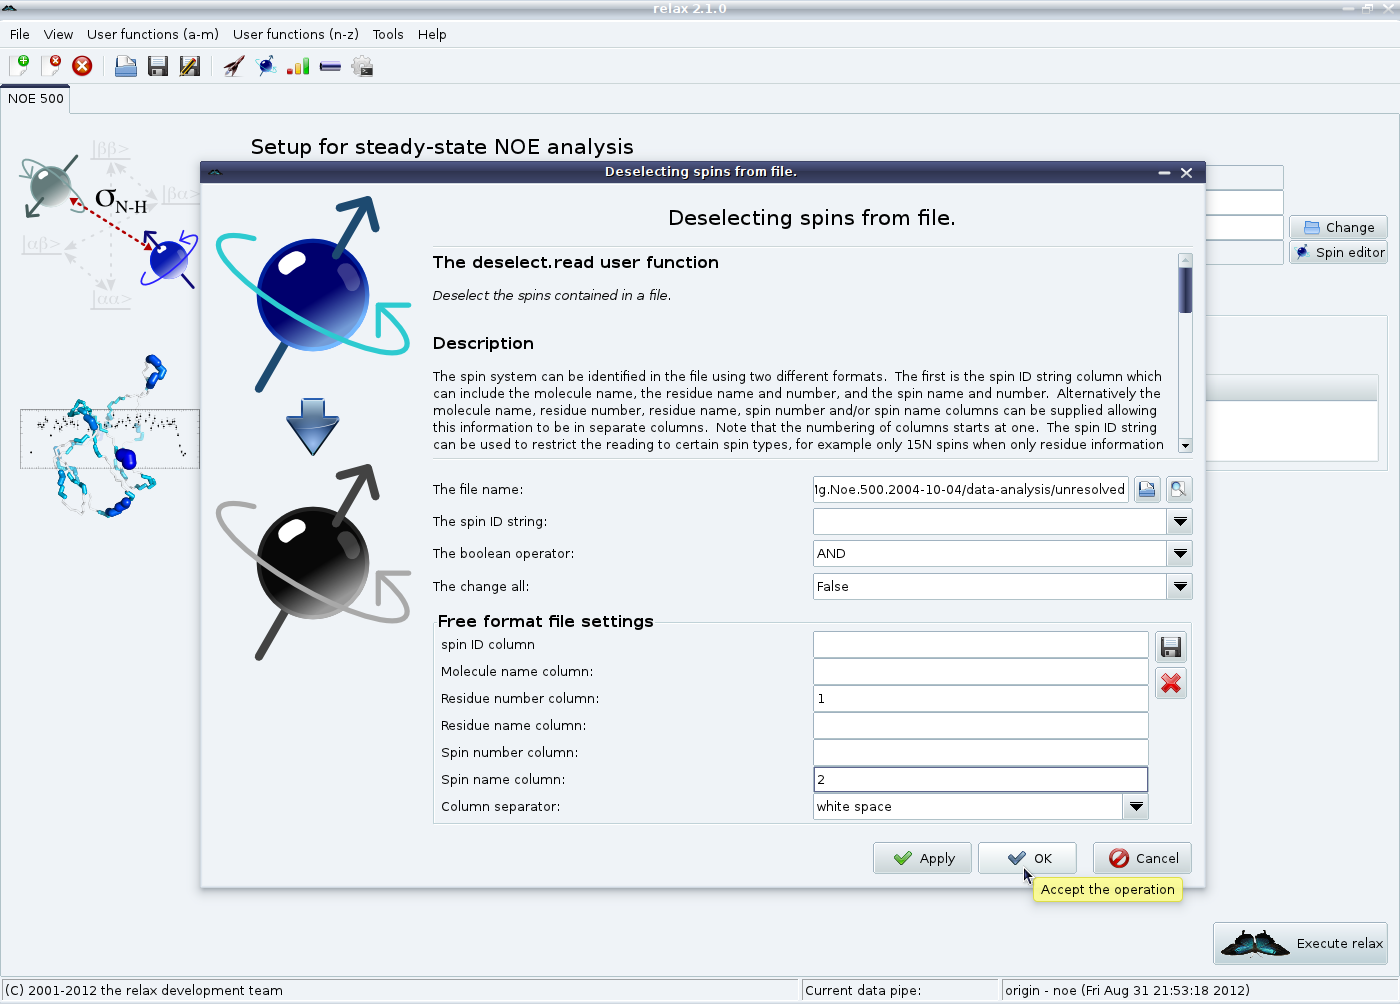
\includegraphics[
      width=0.8\textwidth,
      bb=14 14 1415 1019
    ]
    {graphics/screenshots/noe_analysis/deselect}
  }
\end{minipage}

Alternatively the spin editor window can be reopened and the spins manually deselected by right clicking on them and selecting \gui{Deselect}.
Returning to the spin editor window, you should now see certain spins coloured grey:

\begin{minipage}[h]{\linewidth}
  \centerline{
    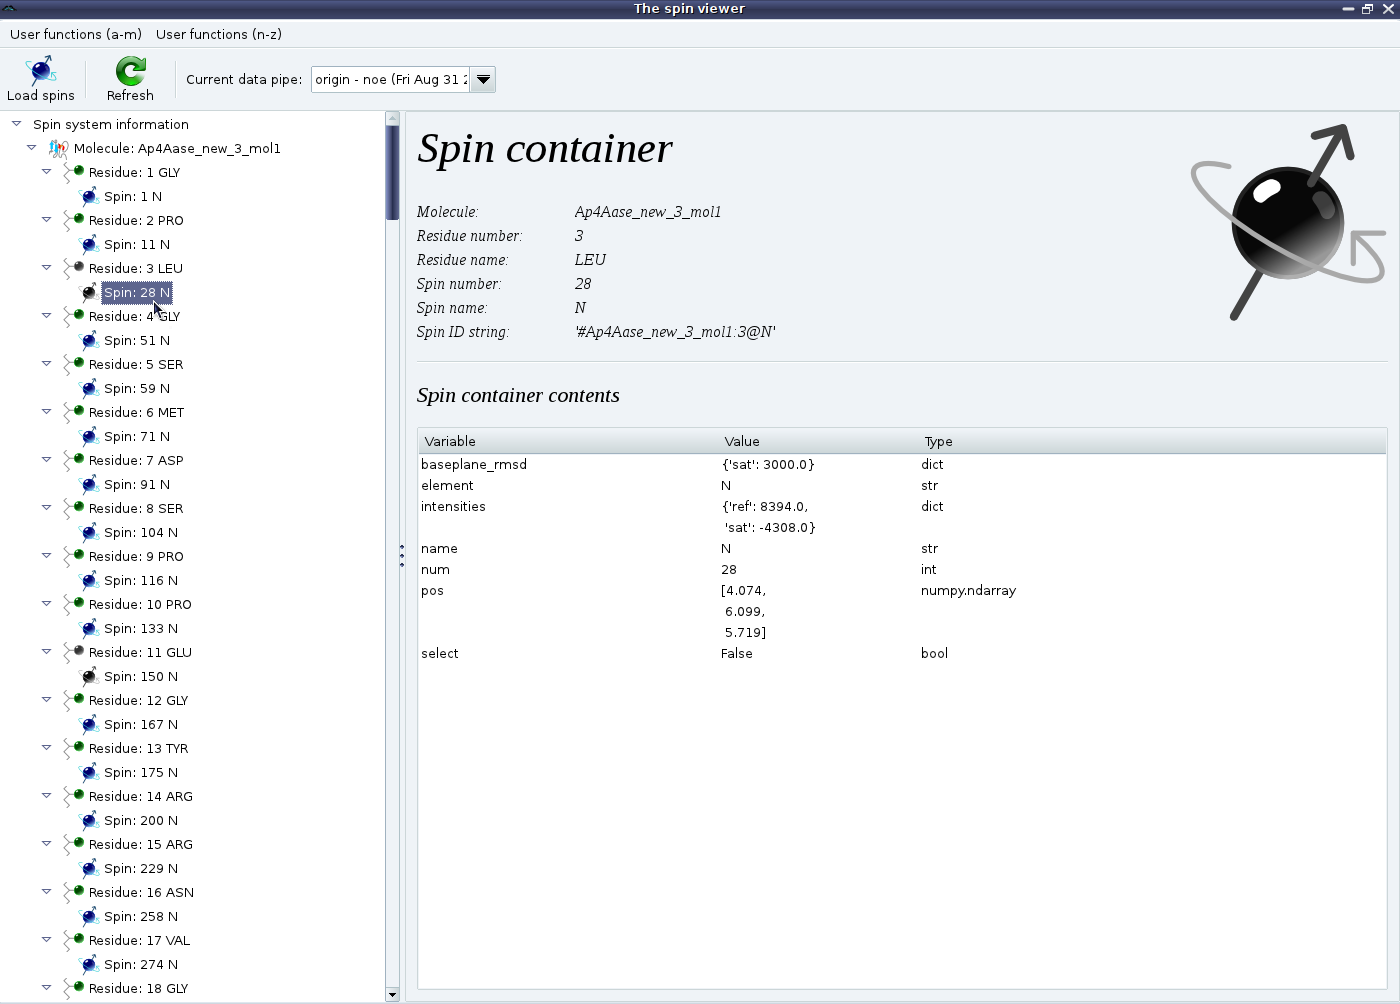
\includegraphics[
      width=0.8\textwidth,
      bb=14 14 1415 1019
    ]
    {graphics/screenshots/spin_viewer/deselect}
  }
\end{minipage}



% The next steps.
%%%%%%%%%%%%%%%%%

\section{The next steps}

This chapter presented the basics of setting up the relax data store, concepts which are needed for all analysis types built into relax.
The next chapters will introduce specific analyses types -- the steady-state NOE, $\Rone$ and $\Rtwo$ relaxation curve-fitting, and the automated full model-free analysis protocol of \citet{dAuvergneGooley07,dAuvergneGooley08b} -- which build on the ideas introduced here.
